
\begin{frame}[c]
  \frametitle{Case I : Diffusion Coefficient and Inventory}
The sensitivity of the peak dose to the reference diffusivity of the 
host rock was analyzed.  In this model, the reference diffusivity of the medium 
was the input parameter used to vary the effective diffusivity in a controlled 
manner. In GoldSim's transport module, the effective diffusion coefficient is 
defined as 

\begin{align}\label{diffcoeff}
  D_{eff} &= n\tau D_{ref}D_{rel} \\ % ?  
       D_{eff} &= ~~\mbox{effective diffusion coefficient }[m^2/s],\nonumber\\
       D_{rel} &= ~~\mbox{relative diffusivity for each isotope in water }[\%],\nonumber\\
       D_{ref} &= ~~\mbox{reference diffusivity in water }[m^2/s],\nonumber\\
       \tau &= ~~\mbox{tortuosity} [\%], \nonumber \\ 
       n &= ~~\mbox{porosity}[\%].\nonumber\\
  \label{GDSEdiff}
\end{align}
\end{frame}

\begin{frame}[c]
  \frametitle{Case I : Diffusion Coefficient and Inventory}
The waste inventory total mass was also altered for each value of the reference 
diffusivity.  That is, the radionuclide inventory in a reference 
\gls{MTHM} of commercial spent nuclear fuel was multiplied by a scalar mass factor.  
It was expected that changing these two parameters in tandem would capture the 
importance of diffusivity in the far field to the repository performance 
as well as a threshold at which the effect of waste inventory dissolution is 
attenuated by solubility limits.
\end{frame}

\begin{frame}[c]
  \frametitle{Case I : Diffusion Coefficient and Inventory}
Finally, in order to isolate the effect of the far field behavior, the waste form 
degradation rate was set to be very high as were the solubility and advective 
flow rate through the  \gls{EBS}. This guaranteed that contaminant flowthrough 
in the near field was unhindered, leaving the far field as the dominant barrier 
to release.
\end{frame}

\begin{frame}[c]
  \frametitle{Case I : Diffusion Coefficient and Inventory}
The forty runs corresponded to eight values of relative diffusivity and five 
values of inventory mass multiplier. That is, the reference diffusivity was varied over the 
eight magnitudes between $ 10^{-8}$ and $10^{-15}$ $[m^2 /s]$ . 
The Mass Factor, the unitless inventory multiplier, was simultaneously varied over 
the five magnitudes between $10^{-4}$ and $10^{1} [-]$. That is, the 
radionuclide inventory was varied between $10^{-4}$ and $10^{1}$ of that in one 
\gls{MTHM} of \gls{SNF}, which is expected to cover the full range of 
inventories in current wasteforms.
\end{frame}

\begin{frame}[c]
  \frametitle{Case I : Diffusion Coefficient and Inventory}
\begin{table}[hbp!]
\centering
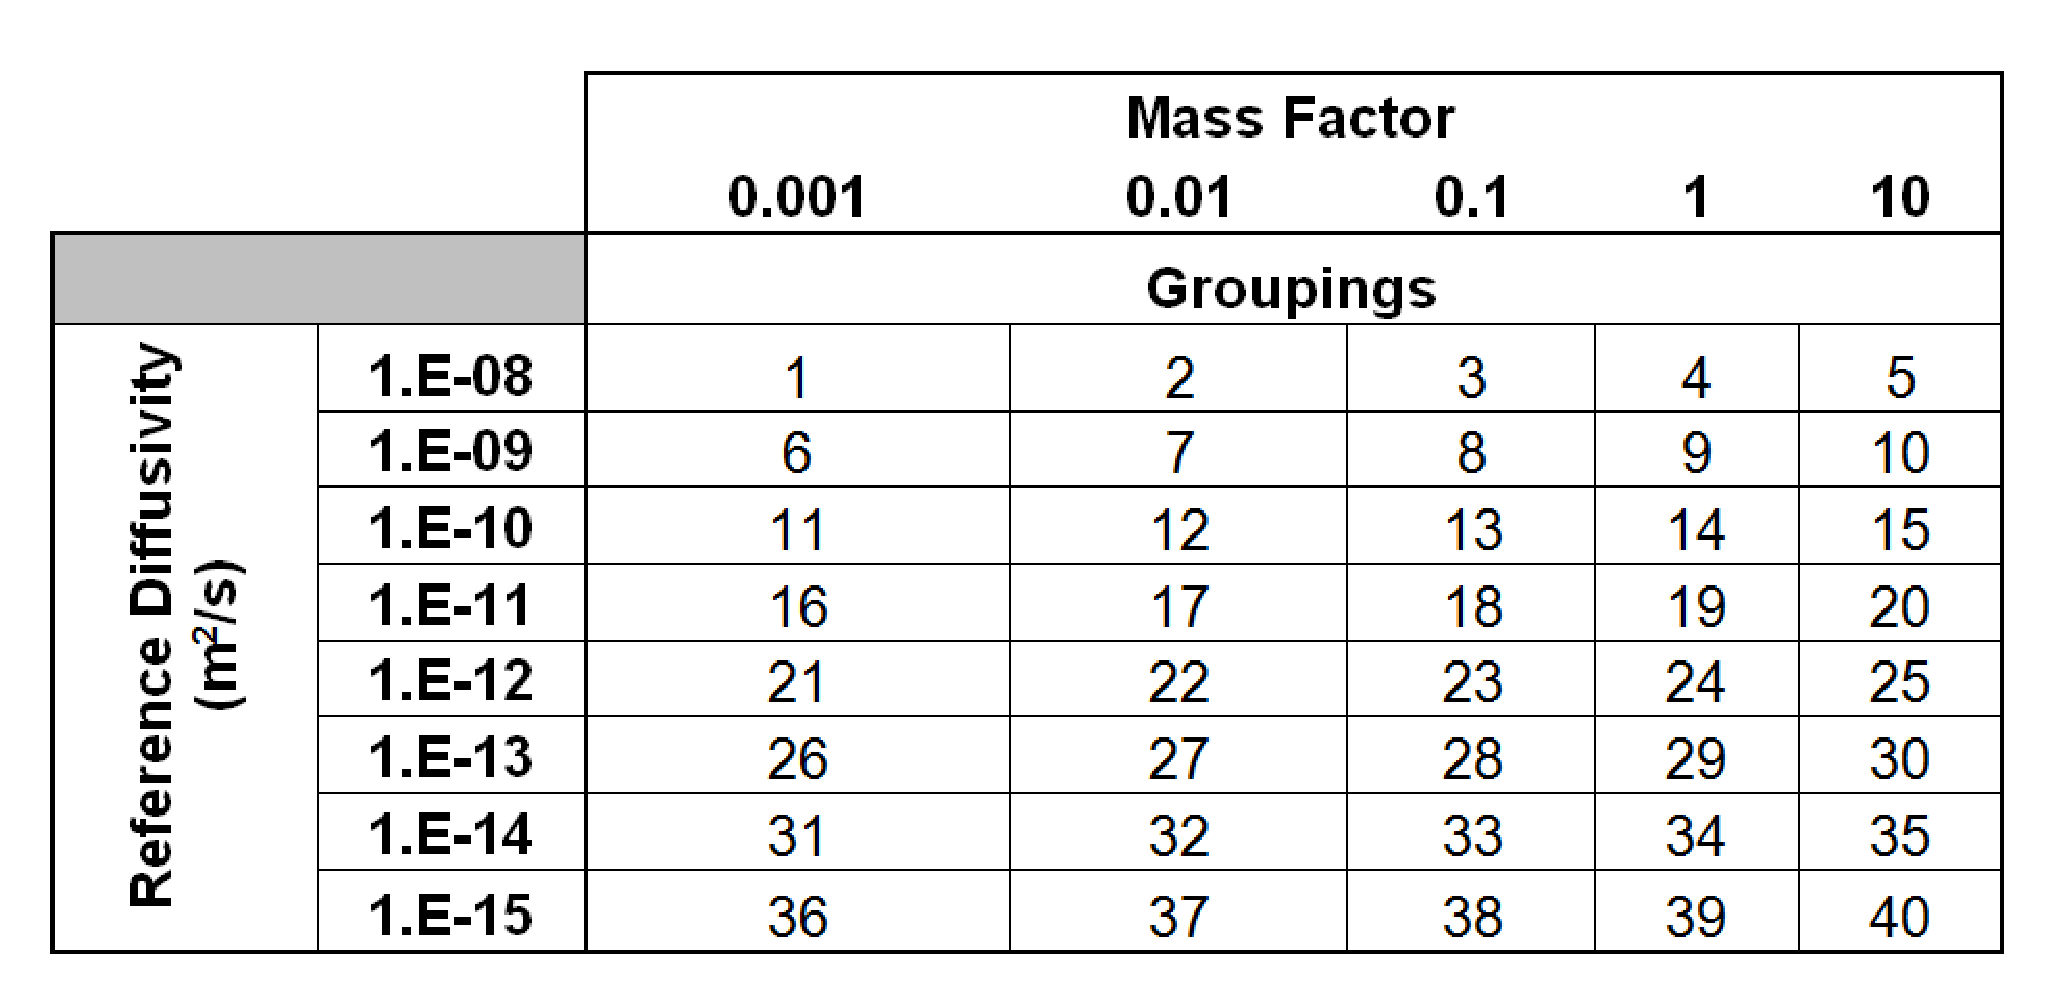
\includegraphics[width=0.7\textwidth]{DiffCoeffAndInvEBSFail/DiffCoeffAndInvGroups.eps}
\caption{Diffusion coefficient and mass factor simulation groupings.}
\label{tab:DiffCoeffAndInvGroups}
\end{table}
\end{frame}

\begin{frame}[c]
  \frametitle{Case I : Diffusion Coefficient and Inventory}
The peak doses due to highly soluble, non-sorbing elements such as $I$ and $Cl$, 
are  proportional to the radionuclide inventory and 
largely directly proportional to the relative diffusivity. This can be seen for 
the cases of $^{129}I$ and $^{36}Cl$ in Figures \ref{fig:DCInvI129}, 
\ref{fig:DCInvI129MF}, \ref{fig:DCInvCl36} and \ref{fig:DCInvCl36MF}.
\end{frame}



\begin{frame}[c]
  \frametitle{Case I : Diffusion Coefficient and Inventory}
\begin{figure}[ht]
\centering
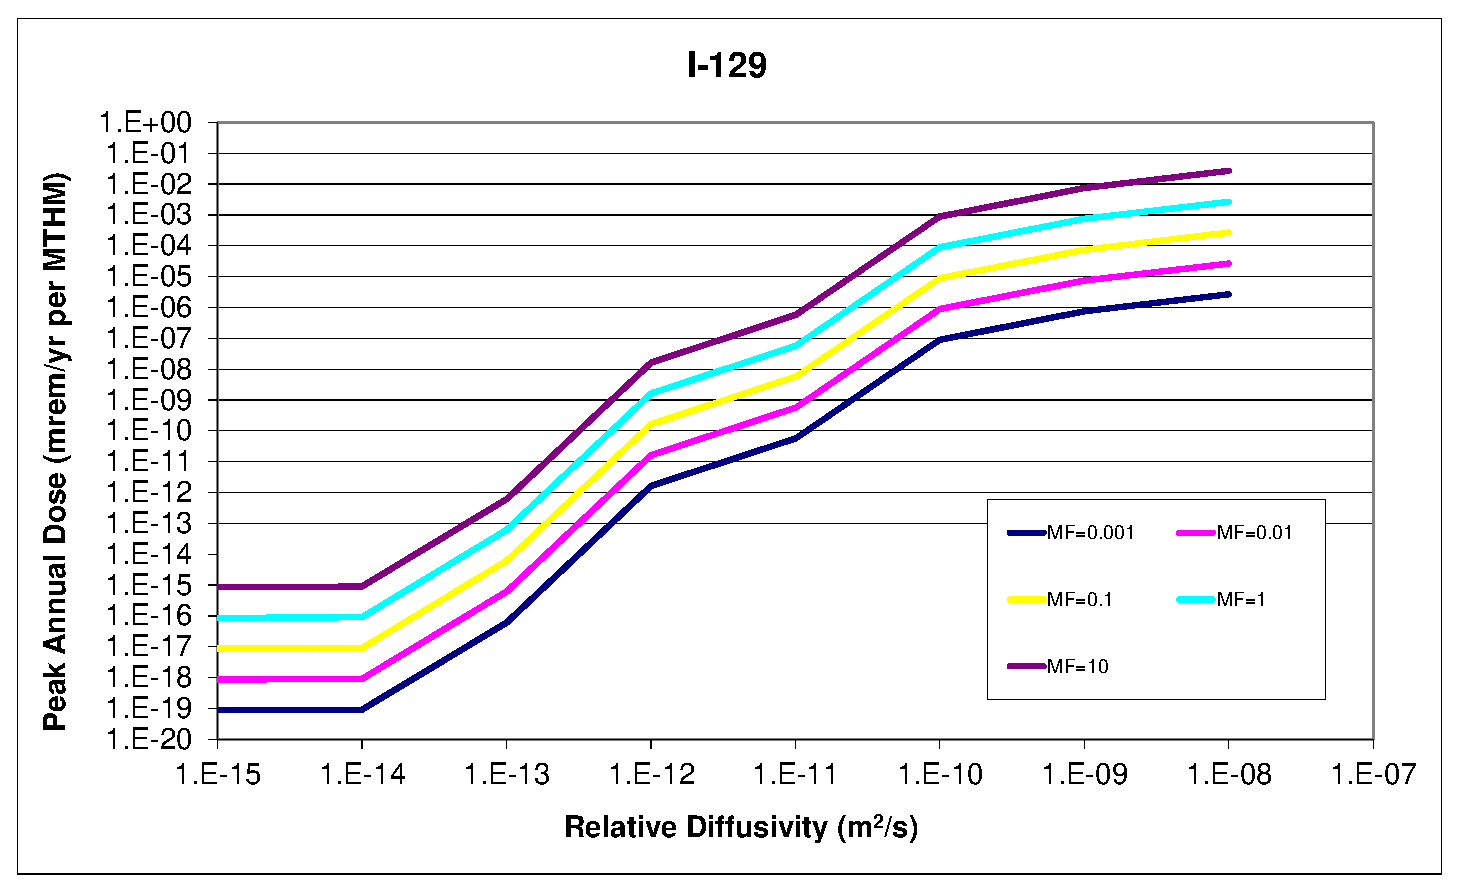
\includegraphics[width=\linewidth]{./DiffCoeffAndInvEBSFail/I-129.eps}
\caption{$^{129}I$ relative diffusivity sensitivity.}
\label{fig:DCInvI129}
\end{figure}
\end{frame}

\begin{frame}[c]
  \frametitle{Case I : Diffusion Coefficient and Inventory}
\begin{figure}[ht]
\centering
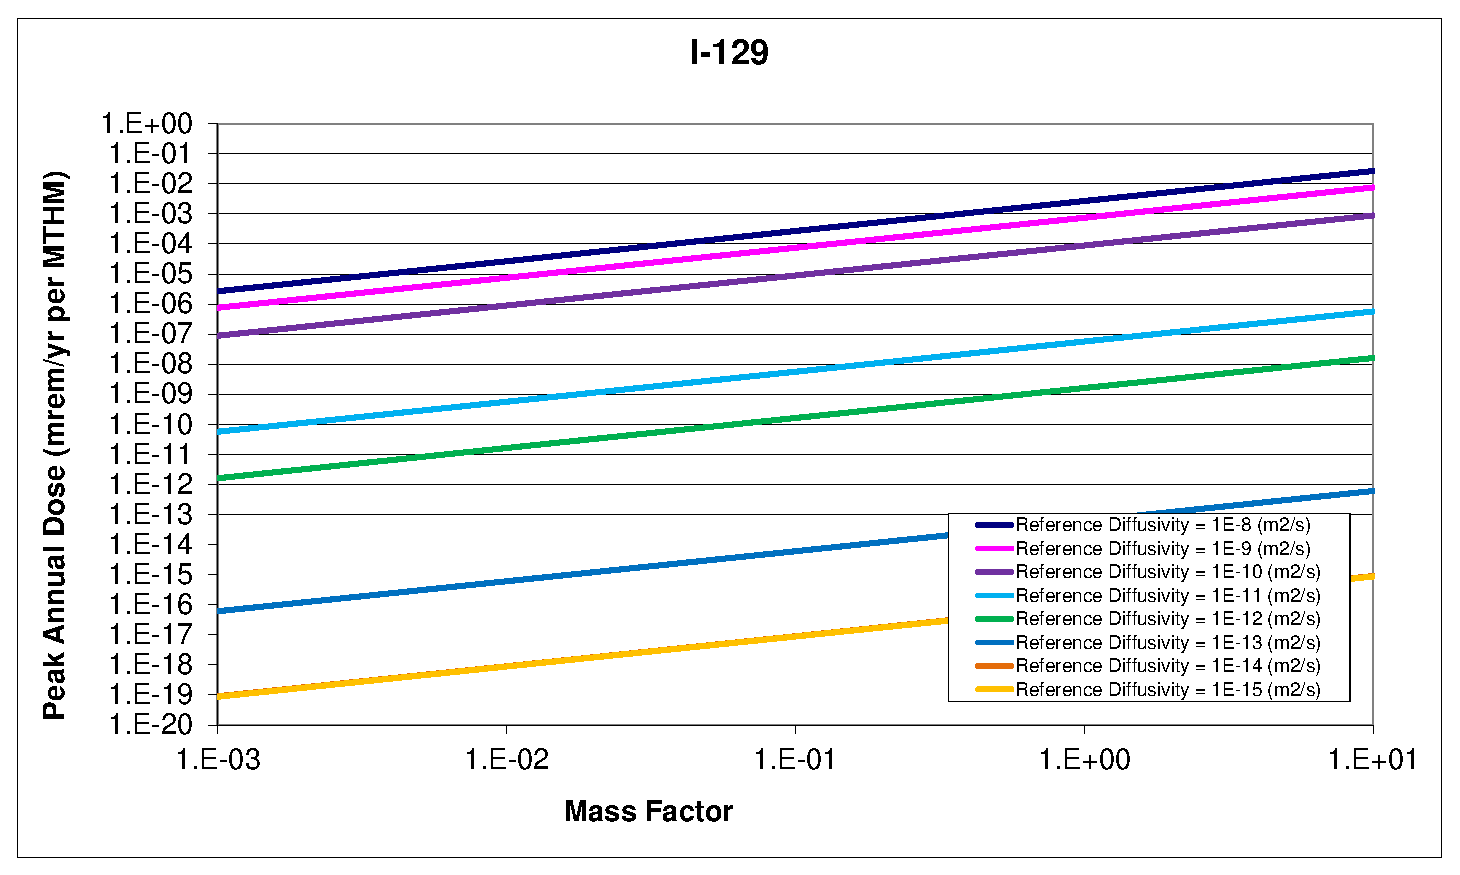
\includegraphics[width=\linewidth]{DiffCoeffAndInvEBSFail/I-129-MF.eps}
\caption{$^{129}I$ mass factor sensitivity.}
\label{fig:DCInvI129MF}
\end{figure}
\end{frame}

\begin{frame}[c]
  \frametitle{Case I : Diffusion Coefficient and Inventory}

\begin{figure}[ht]
\centering
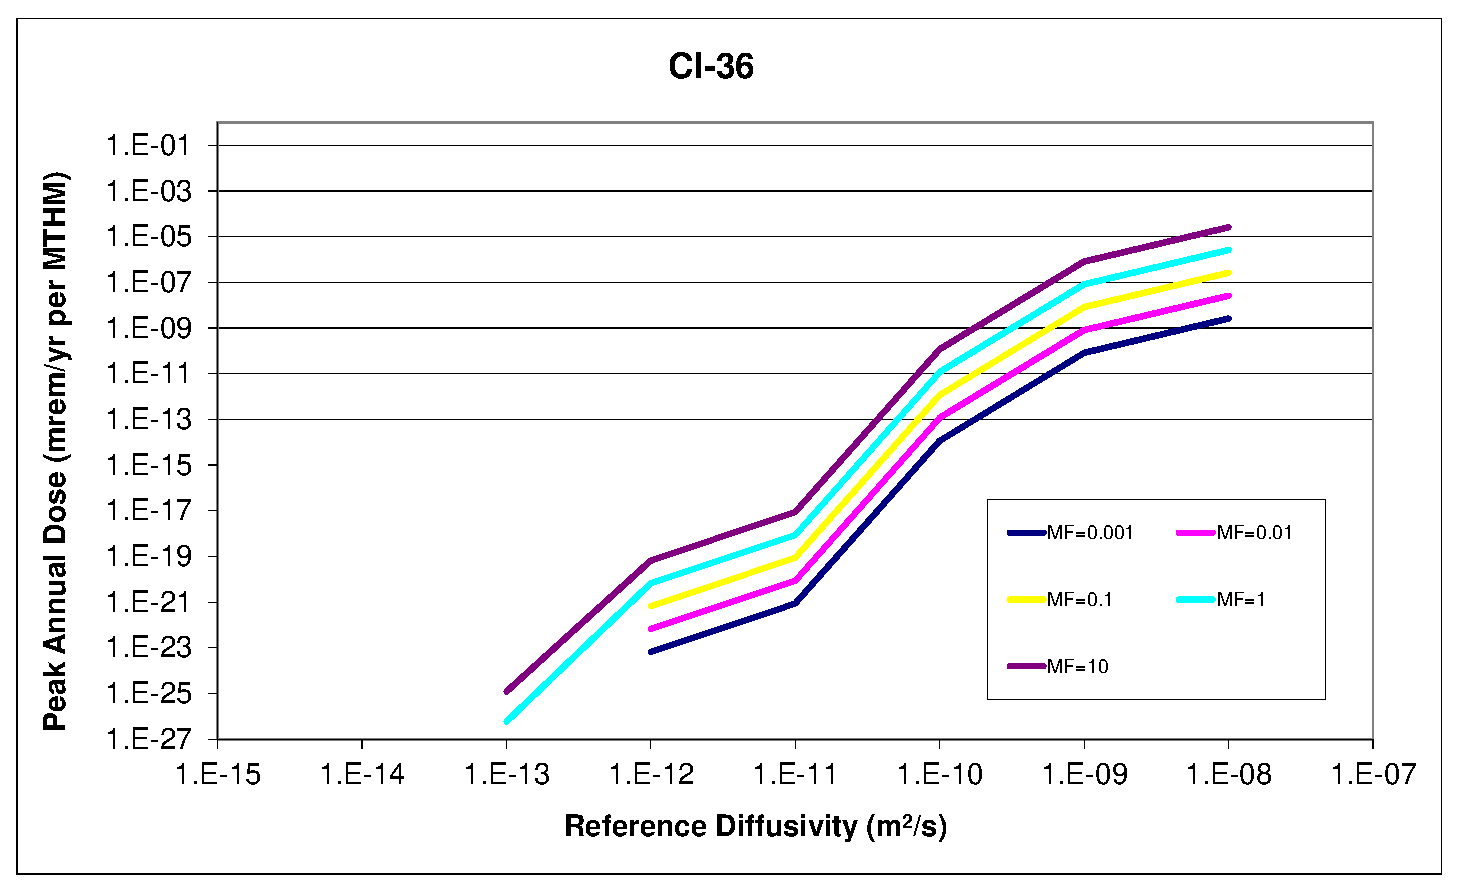
\includegraphics[width=\linewidth]{DiffCoeffAndInvEBSFail/Cl-36.eps}
\caption{$^{36}Cl$ relative diffusivity sensitivity.}
\label{fig:DCInvCl36}
\end{figure}
\end{frame}

\begin{frame}[c]
  \frametitle{Case I : Diffusion Coefficient and Inventory}

\begin{figure}[ht]
\centering
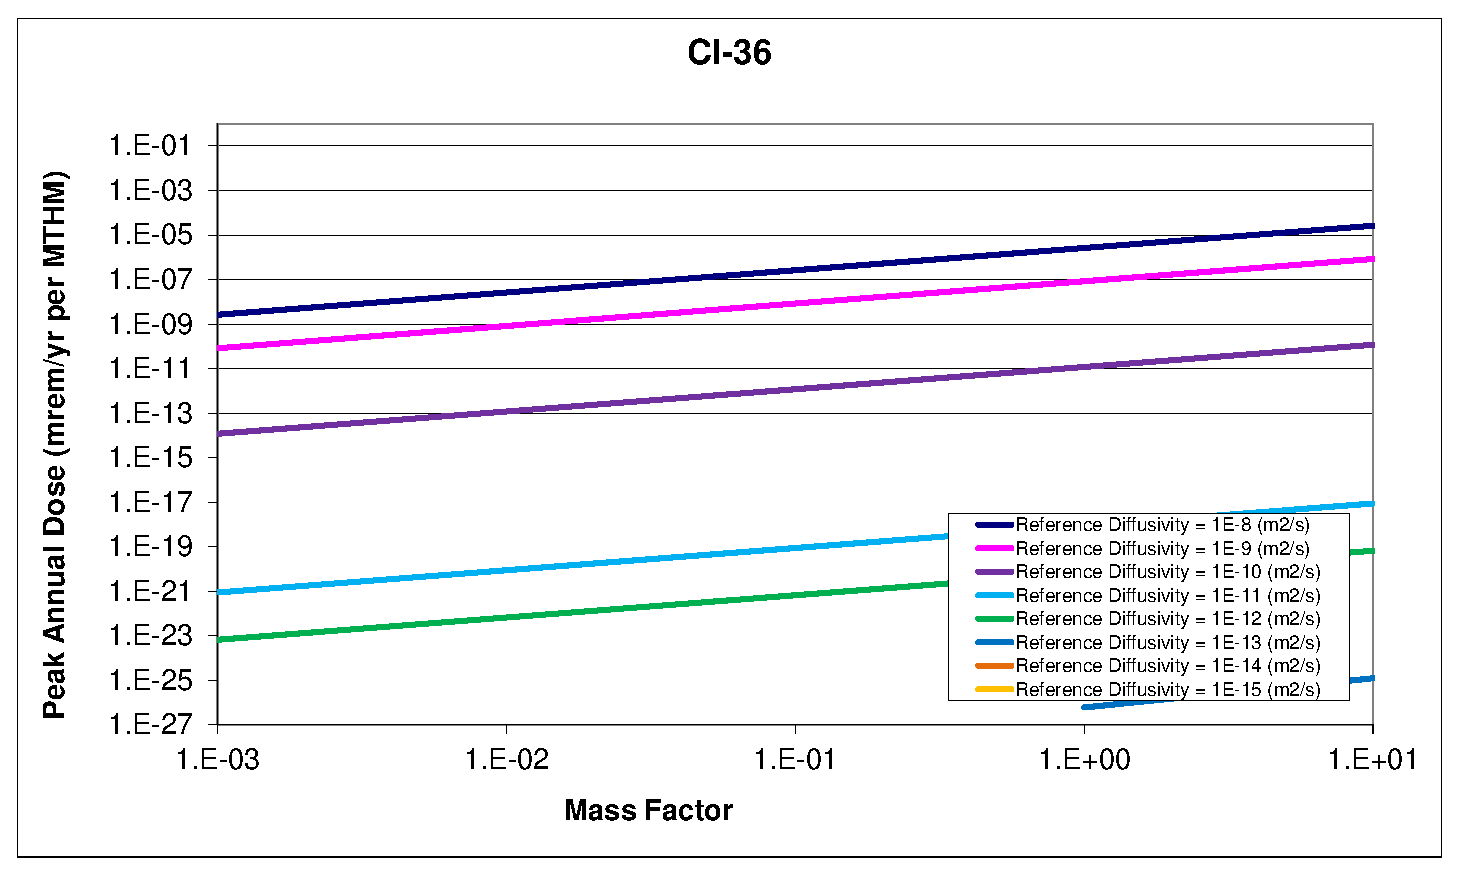
\includegraphics[width=\linewidth]{DiffCoeffAndInvEBSFail/Cl-36-MF.eps}
\caption{$^{36}Cl$ mass factor sensitivity.}
\label{fig:DCInvCl36MF}
\end{figure}
\end{frame}


\begin{frame}[c]
  \frametitle{Case I : Diffusion Coefficient and Inventory}

\begin{figure}[ht!]
\centering
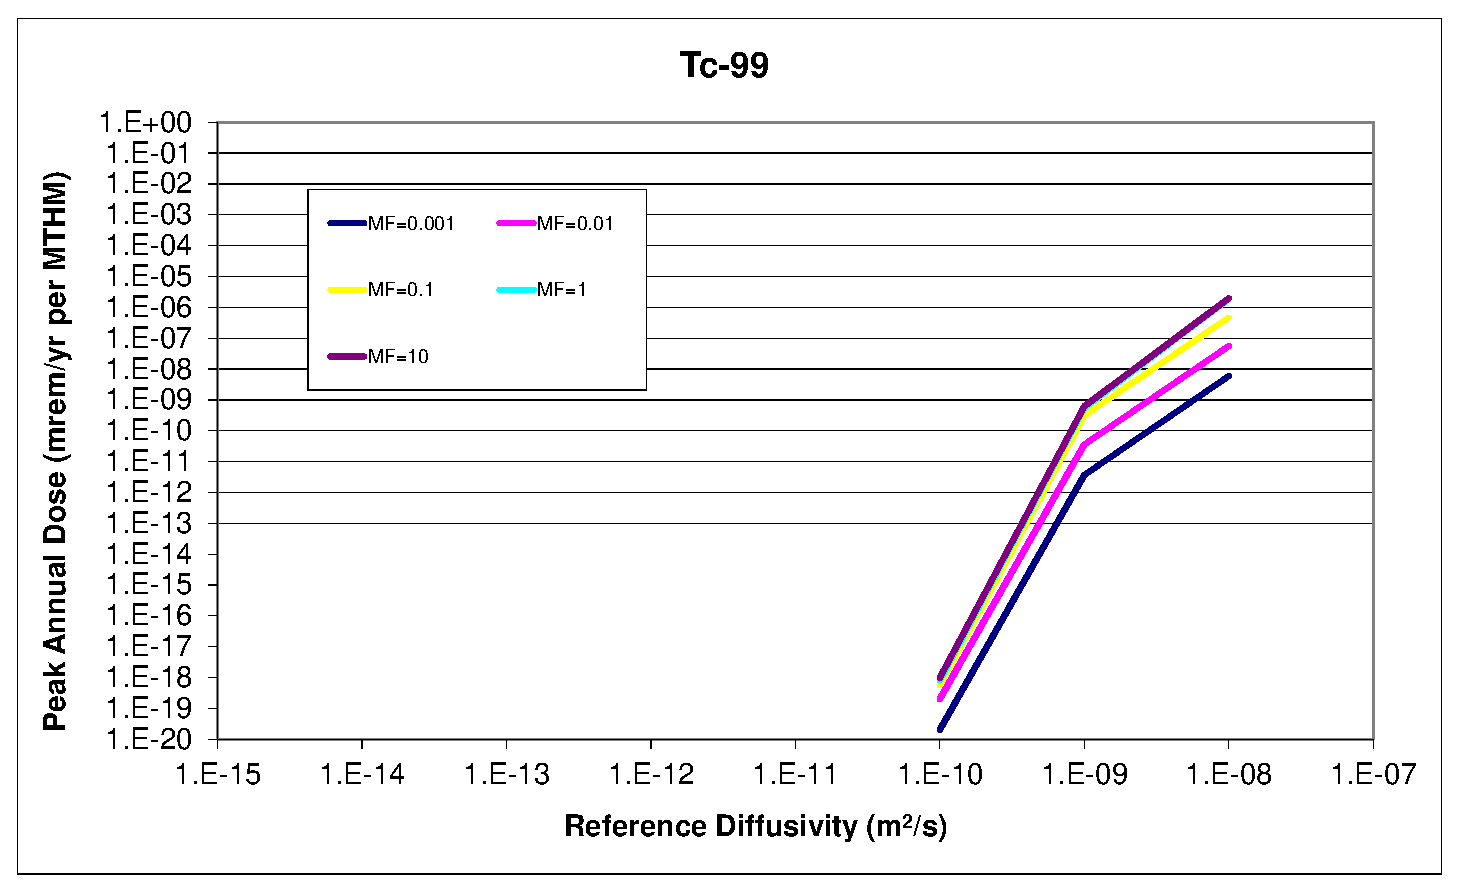
\includegraphics[width=\linewidth]{DiffCoeffAndInvEBSFail/Tc-99.eps}
\caption{$^{99}Tc$ relative diffusivity sensitivity.} 
\label{fig:DCInvTc99}
\end{figure}
\end{frame}

\begin{frame}[c]
  \frametitle{Case I : Diffusion Coefficient and Inventory}

\begin{figure}[ht!]
\centering
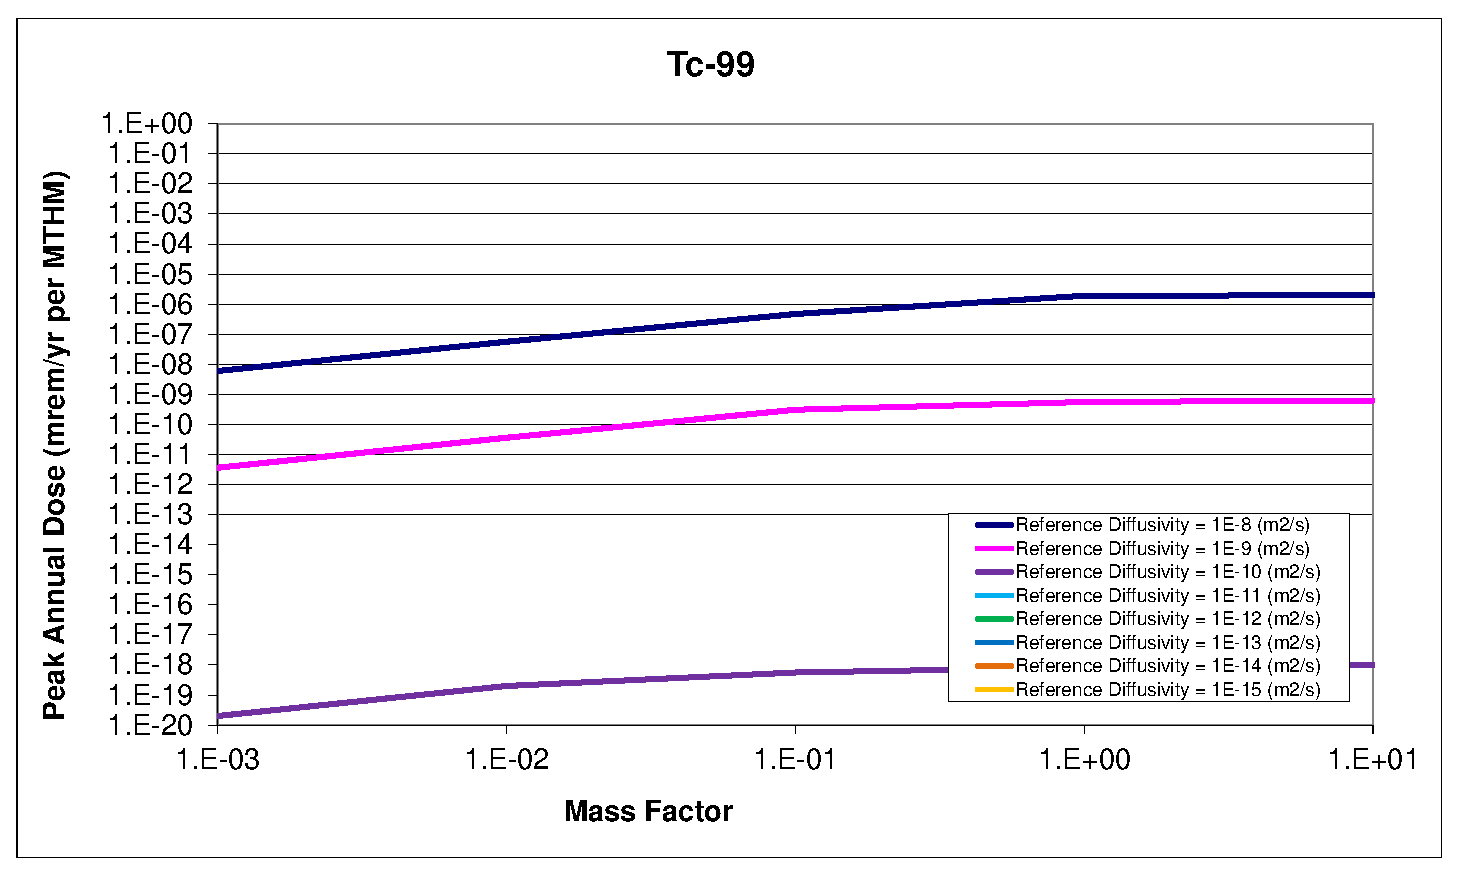
\includegraphics[width=\linewidth]{DiffCoeffAndInvEBSFail/Tc-99-MF.eps}
\caption{$^{99}Tc$ mass factor sensitivity.}
\label{fig:DCInvTc99MF}
\end{figure}
\end{frame}

\begin{frame}[c]
  \frametitle{Case I : Diffusion Coefficient and Inventory}


\begin{figure}[ht!]
\centering
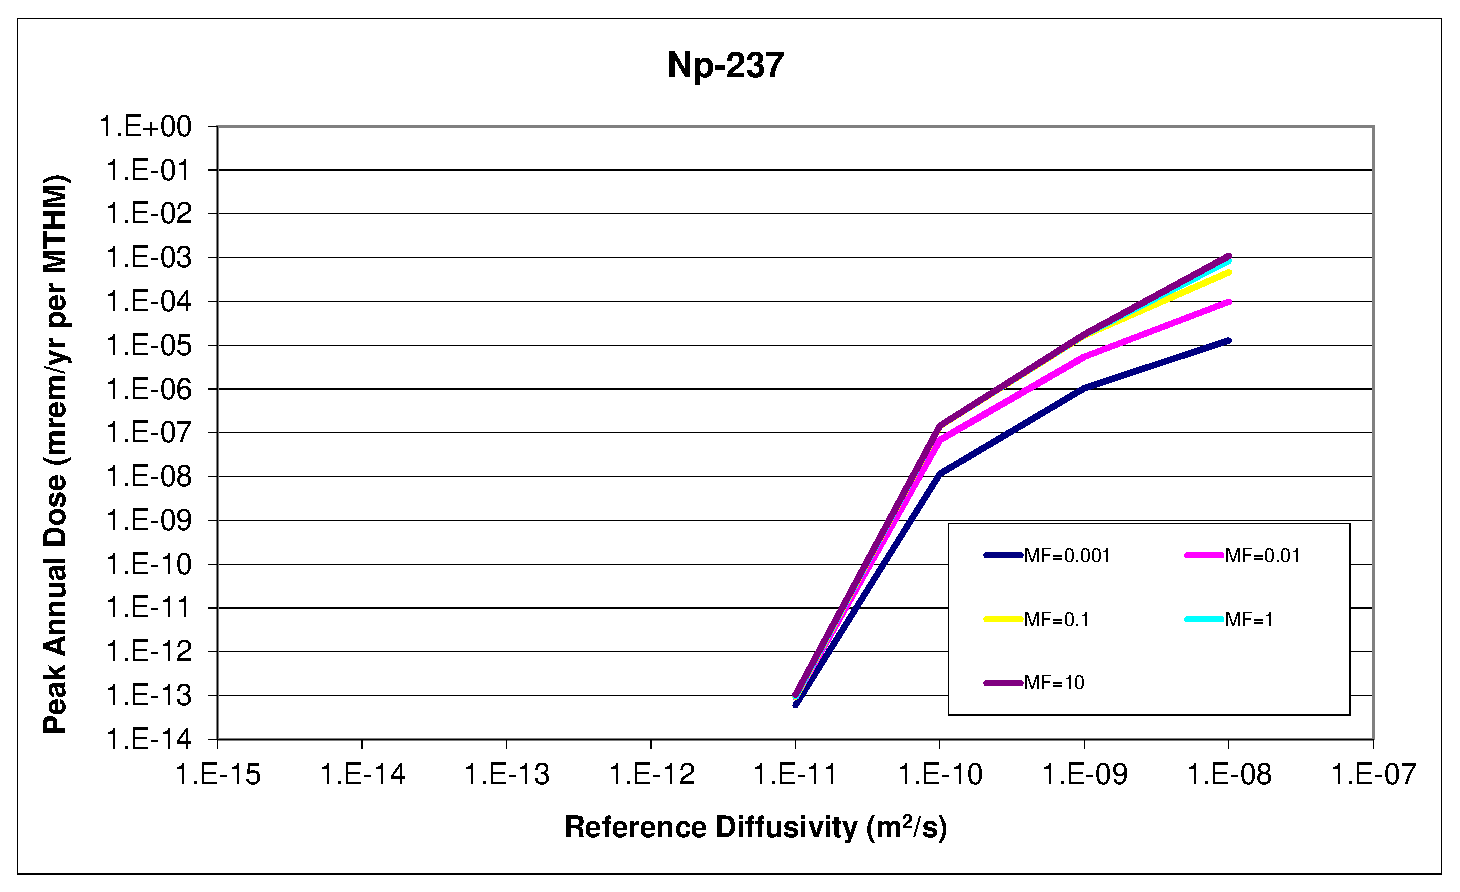
\includegraphics[width=\linewidth]{DiffCoeffAndInvEBSFail/Np-237.eps}
\caption{$^{237}Np$ relative diffusivity sensitivity.} 
\label{fig:DCInvNp237}
\end{figure}
\end{frame}

\begin{frame}[c]
  \frametitle{Case I : Diffusion Coefficient and Inventory}

\begin{figure}[ht!]
\centering
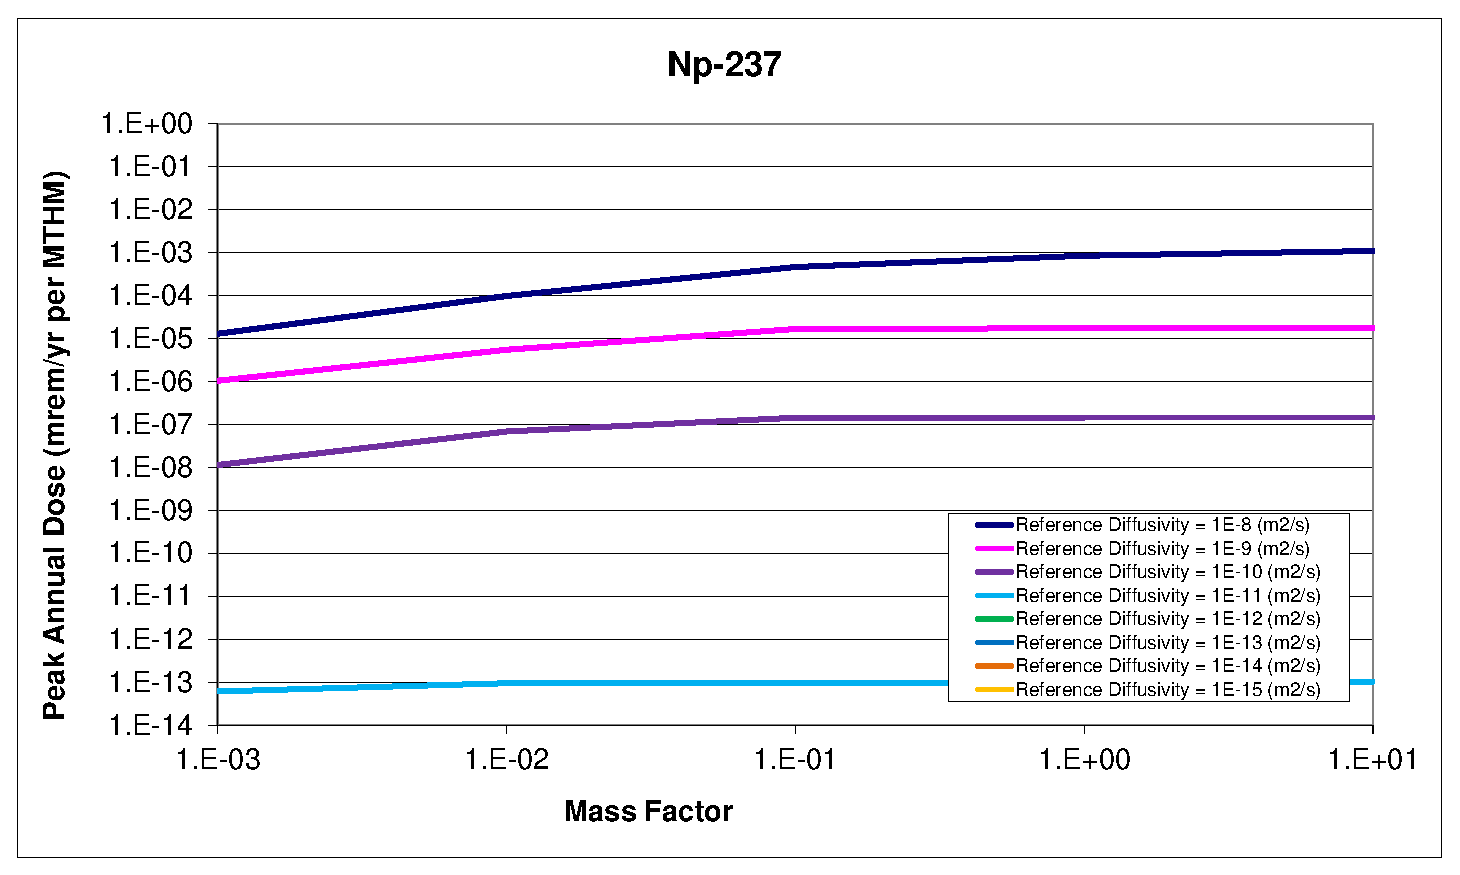
\includegraphics[width=\linewidth]{DiffCoeffAndInvEBSFail/Np-237-MF.eps}
\caption{$^{237}Np$ mass factor sensitivity.}
\label{fig:DCInvNp237MF}
\end{figure}
\end{frame}
